%%%%%%%%%%%%%%%%%%%%%%% file template.tex %%%%%%%%%%%%%%%%%%%%%%%%%
%
% This is a general template file for the LaTeX package SVJour3
% for Springer journals.          Springer Heidelberg 2010/09/16
%
% Copy it to a new file with a new name and use it as the basis
% for your article. Delete % signs as needed.
%
% This template includes a few options for different layouts and
% content for various journals. Please consult a previous issue of
% your journal as needed.
%
%%%%%%%%%%%%%%%%%%%%%%%%%%%%%%%%%%%%%%%%%%%%%%%%%%%%%%%%%%%%%%%%%%%
%

\RequirePackage{fix-cm}
%
\documentclass{svjour3}                     % onecolumn (standard format)
%\documentclass[smallcondensed]{svjour3}     % onecolumn (ditto)
%\documentclass[smallextended]{svjour3}       % onecolumn (second format)
%\documentclass[twocolumn]{svjour3}          % twocolumn
%
\smartqed  % flush right qed marks, e.g. at end of proof
%
\usepackage{graphicx}
\usepackage{amsmath}
\usepackage{enumitem}
%
% \usepackage{mathptmx}      % use Times fonts if available on your TeX system
%
% insert here the call for the packages your document requires
%\usepackage{latexsym}
% etc.
%
% please place your own definitions here and don't use \def but
% \newcommand{}{}
%
% Insert the name of "your journal" with
% \journalname{myjournal}
%
\begin{document}

\title{EasyPot: an Interactive Modeling System for Pottery Design in Virtual Reality%\thanks{Grants or other notes
%about the article that should go on the front page should be
%placed here. General acknowledgments should be placed at the end of the article.}
}
%\subtitle{Do you have a subtitle?\cite{Jacob2008Reality}  \\ If so, write it here \cite{website:unity3d}}

%\titlerunning{Short form of title}        % if too long for running head

\author{Zihan Gao         %\and
        %Guangsheng Feng %etc.
}

%\authorrunning{Short form of author list} % if too long for running head

\institute{Zihan Gao \at
              145 Nantong Street, Harbin, China \\
              Tel.: +86-155-9088-5326\\
              \email{gao\_zihan@126.com}           %  \\
%             \emph{Present address:} of F. Author  %  if needed
           \and
           S. Author \at
              second address
}

\date{Received: date / Accepted: date}
% The correct dates will be entered by the editor


\maketitle

\begin{abstract}
We present EasyPot, an interactive virtual reality (VR) modeling system that allows novice users to create virtual pottery works by bimanual interactions via hand-held motion controllers.
Our system consists of two major components: an automatic mesh generator and an interactive model editor.
The mesh generator can procedurally generate a realistic clay mesh by adding Perlin Noise. With the interactive pottery model editor, the user can shape the virtual clay in realtime intuitively to design virtual pots.
The virtual pots created by our system can be exported as OBJ files and used for 3D printing.
The results of our user study have shown that our system is easier to use and allows more creativity compared with desktop modeling systems and touchscreen based systems. Users without real life pottery experience and 3D modeling knowledge can easily create pottery works with our system.

%Insert your abstract here. Include keywords, PACS and mathematical
%subject classification numbers as needed.
\keywords{Virtual pottery \and Natural user interfaces \and Mesh deformation}
% \PACS{PACS code1 \and PACS code2 \and more}
% \subclass{MSC code1 \and MSC code2 \and more}
\end{abstract}

%%% Introduction

\section{Introduction}
\label{sec:1}
%[CAD tools - hard to use]
Pottery is one of the oldest inventions in many civilizations in human history for thousands of years, which is made by shaping clay into heterogeneous forms.
In recent years, emerging technologies such as 3D printing introduces a new way of pottery design, enabling people to fabricate pots in a digital way with the help of Computer Aided Design (CAD) software and 3D printers.
Professional CAD tools, such as Maya\cite{website:maya} and 3ds Max\cite{website:3dmax}, provide powerful toolsets and rich features for 3D modeling pipeline.
However, for novice users who are not professional 3D artists, these systems are formidable to learn due to complex user interfaces. 
This kind of systems limits the creativity of novice users, since it is quite challenging for them to master the tools in a short period of time.
There are several CAD systems which are specifically developed for pottery design \cite{koutsoudis2009qp,kumar2011wheel}, which can generate 3D meshes based on the values from user keyboard and mouse input. Although having simplified user interfaces comparing with professional tools, the experience of these systems is not intuitive and the operations are far different from the workflow in reality.

%[in-air interaction system - freehand, lacks robustness, feedback and reality]
To address this situation, some camera-based virtual pottery systems have been developed \cite{ramani2015gesture,murugappan2013handy,han2014virtual}, which provides natural and intuitive user interfaces, allowing users to design pots via freehand interactions.
These works indeed provide a gentle learning curve, however, they have some common limitations.
First, freehand interactions from depth cameras lacks robustness due to jittering, whose inaccuracy hinders work efficiency and user experience severely.
Second, freehand interaction lacks haptic feedback, making it difficult for users to perceive if they have touched anything in VR environments.
In addition, some features of clay, namely shape irregularity, thickness etc., are missing from these systems, undermining realistic look and feel in the pot design process.

%[design goals: 1. simple 2. robust/realistic]
In this paper, we present EasyPot, a VR system that allows users to design virtual pottery models from their hand movement using hand-held motion controllers. There are two major design goals for EasyPot:

\begin{itemize}
%[easy]
\item Provide a simple and intuitive interface for novice users to learn virtual pottery skills with minimum cognitive load.
%[robust realistic]
\item Design a robust virtual pottery system on VR devices that can generate realistic clay meshes and provide refined haptic feedbacks based on bimanual spatial interactions.
\end{itemize}

%[design considerations: 1.HCD 2. RBI]
Oviatt \cite{oviatt2006human} concluded that human-centered design can minimize users’ cognitive load, which effectively frees up mental resources for performing better while also remaining more attuned to the world around them.
%% TODO
So we take the human-centered design approach, which models users’ natural behavior so that interfaces can be more intuitive, easier to learn, and freer of performance errors.
In addition, Jacob et al. \cite{Jacob2008Reality} summarized that the designer's goal should be to allow the user to perform realistic tasks realistically, to provide additional non real-world functionality, and to use analogies for these commands whenever possible.
Hence, while we design our system based on pottery creation process in reality to minimize the effort, we should provide convenient functionalities in our system for efficiency.

%[contributions]
The main contributions of our works are:

\begin{itemize}
\item Present a virtual pottery system which can generate pot models from user spatial interaction for 3D printing.
\item Propose a virtual pottery workflow by introducing simple and intuitive user interfaces for modeling, enabling novice users to understand and learn pottery production pipeline.
\item Conduct an user study showing the comparison results among three modeling systems. The results have shown that our system is easier to use compared with traditional 3D modeling tools and is more intuitive and immersive than touchscreen based interfaces.
\end{itemize}


%%%

\section{Related Work}
\label{sec:2}

\subsection{Bimanual Interaction}
\label{sec:2.1}
Bimanual interaction has been a popular research field, which can accomplish a variety of tasks in both physical and virtual environments.
In terms of mechanisms, bimanual interaction can be classified into two categories: bare-hand based interactions and instrument based interactions.

There are a great number of research efforts \cite{walter2014cuenesics,cui2016exploration,ramani2015gesture,murugappan2013handy,han2014virtual} on bare-hand based interactions using depth camera such as Kinect, Leap Motion etc.
Cuenestics \cite{walter2014cuenesics} is a design space for hand-gesture based mid-air selection techniques using a depth camera Kinect, where users can select contents on interactive public displays with their gesture input.
Cui et al. \cite{cui2016exploration} proposed a modeling system with natural free-hand interaction using a Leap Motion controller, allowing users to grab and manipulate objects with one or two hands intuitively.
While these works provided accessibility to users, the limitations are obvious as well: The input is not always accurate due to many factors such as lighting condition and occlusion, which might cause user frustration.
In addition, these methods do not provide haptic feedbacks, which hinders the realistic feel for users.

Unlike bare-hand based interactions, instrument based interactions provide more control precision, haptic feedback and unambiguity.
Surface Drawing \cite{schkolne2001surface} is a system for creating organic 3D shapes using tangible tools such as gloves, where users can define strokes with the path of hands wearing gloves.
Hinckley et al. \cite{hinckley1998two} did a research on two-handed virtual manipulation with a point design of a prop-based system, which allows users to view a cross section of a brain with interface props.
These works have a common problem that the usage of these instruments are limited to a lab context that very few users can access.
%
With the commercialization of gaming devices, some motion controllers such as Wii Remote and HTC Vive have become accessible to consumers, which are also used in scientific studies for 3D user interfaces \cite{wingcrave2010wii,niehorster2017accuracy}.
%
In our project, HTC Vive system is used in our system, which provides precision, haptic feedback and well accessed by consumers.

\subsection{Art and Design Tools in VR}
\label{sec:2.2}
Virtual Reality has shown great potential for art and design, which not only provides immersive and intuitive interfaces for user, but also creates new art medium, new art form and novel experience\cite{laviola20113d}.

CavePainting \cite{keefe2001cavepainting} is a 3D artistic medium in a fully immersive environment, which enables artists to create spatial paintings with physical props and gestures. Agrawala et al.\cite{agrawala19953d} developed an interface for painting on polygon meshes using a 6DOF space tracker, which provides a natural force-feedback for painting, allowing users to place colors on meshes intuitively. MAI Painting Brush++ \cite{otsuki2017brush} is a brush device for virtual painting of 3D virtual objects, where users could take a physical object in the real world and apply virtual paint to it with visual and haptic feedback.

Virtual Clay \cite{mcdonnell2001virtual} is a sculpture framework based on subdivision solids and physics-based modeling, which is equipped with natural, haptic based interaction, providing users with a realistic sculpting experience. Sheng et al. \cite{sheng2006interface} proposed an interface for virtual 3D sculpting, which uses camera-based motion tracking technology to track passive markers on the fingers and prop, enabling users to apply operations such as deforming, smoothing, pasting and extruding.

\subsection{Virtual Pottery Systems}
\label{sec:2.3}


Several systems have been specifically developed for virtual pottery design. Unlike some sculpting systems mentioned above, virtual pottery systems allow rotational symmetry, and much easier for novice users.

Qp \cite{koutsoudis2009qp} was a tool for generating 3D pottery models, which can produce a collection of random 3D ancient greek vessels.
Based on number-theoretic techniques, Kumar et al. \cite{kumar2011wheel} presented a system for creating digital potteries including thick-walled potteries as well, which resembles pottery works in real life.
While these systems can generate heterogeneous pottery models efficiently, their user interfaces are limited to traditional keyboard and mouse input, which are not helpful for training users to understand the pottery creation process.

%%CHINA korida1997interactive
Handy-Potter \cite{murugappan2013handy} was a rapid 3D creation tool, which tracks user skeletons with depth sensing camera Kinect, enabling users to create potteries using hands and arms.
%%CAD ramani2015gesture
Han et al. \cite{han2014virtual} presented an audiovisual interface, where hand motions are translated into musical sound.
In AR Pottery \cite{han2007ar}, augmented reality has been applied to pottery design, with which users can deform a virtual pottery using a marker held by hand.
Although with these systems users could create some virtual pottery works, the actions applied are quite different from real life pottery making process. Thus, users cannot learn the actual pottery process from using these systems effectively.

%[design consideration - EDUCATION!!!]
In contrast to existing works, our system provides a novel pottery creation workflow in virtual reality which lets user shape pottery through two-handed spatial interactions, helping novice users to understand and learn real life pottery skills.




\section{System Overview}
\label{sec:3}

\subsection{System Architecture}
\label{sec:3.1}

TODO

%%% architecture
\begin{figure*}
\includegraphics[width=\textwidth]{arc.pdf}
\caption{The system architecture of EasyPot.}
\label{fig:1}
\end{figure*}



\subsection{Workflow}
\label{sec:3.2}
The pottery creation process on a pottery wheel is called "throwing", where a ball of clay is placed in the centre of a turntable wheel-head, and shaped by a potter.
To illustrate the pipeline of pottery creation in our system, an example workflow using EasyPot is described as follows.

When a user starts to use EasyPot, a realistic clay mesh is automatically generated with Perlin noise. (Figure \ref{fig:2}a, Section \ref{sec:4.1})
Similar to the operation in reality, the user first need to use both hands to make the irregular clay shape into perfect rotational symmetry, which is called \textit{centring}. (Figure \ref{fig:2}b, Section \ref{sec:4.2.1})
The user can control the thickness of the clay (i.e. \textit{opening}) by pressing down the clay to create a hollow in the clay (Figure \ref{fig:2}c), 
and then draw up the walls with two hands moving up together (i.e. \textit{pulling}), controlling the height of the clay. (Figure \ref{fig:2}d, Section \ref{sec:4.2.2})
The system not only allows mesh deformation ( Figure \ref{fig:2}e, Section \ref{sec:4.2.3}) with different deformation range parameters but also mesh smoothing (Figure \ref{fig:2}f, Section \ref{sec:4.2.4}), where the user can remove sharp features in the pot to get ideal shape.
After the creation process is finished, the user can export the pottery model as an OBJ file, which can be used for 3D printing.

%%% Fig 2
\begin{figure*}
\includegraphics[width=\textwidth]{fig2.pdf}
\caption{(a) The automatically generated clay mesh with Perlin Noise. (b) The mesh is shaped into rotational symmetry by using both hands. (c) The user controls the thickness of the mesh by pressing down the clay. (d) The user controls the height of the mesh by drawing up the clay wall.(e) The deformation range can be adjusted to get varied deformation effect on different parts. (f) The sharp features on the upper part can be removed by mesh smoothing.}
\label{fig:2}
\end{figure*}

\section{Interactive Modeling System for Pottery Design in VR}
\label{sec:4}

\subsection{Mesh Generation}
\label{sec:4.1}

Most of virtual pottery systems approximate the initial shape of pottery clay as a primitive cylinder shape \cite{han2007ar,ramani2015gesture,Vinayak2016Extracting}. While this approach is simple to implement, it ignores subtle details of clay in real life, whose irregularity needs to be dealed with during the creation process. Unlike the existing systems, we first approximate the initial clay on the pottery wheel as a blending shape of cylinder and semi-ellipsoid, then adding Perlin noises to mimic the irregular clay in reality.

\paragraph{Basic clay} We describe the clay mesh as a series of circular sections in different heights, whose resolution can be defined by axis segments $s_{a}$ and height segments $s_{h}$. Given radius $r$ and height $h$, our system can generate primitive mesh of cylinder and semi-ellipsoid respectively (Figure \ref{fig:3}).
For each vertex in the mesh, we use a $m \times n$ matrix $M$ to store radius values, where number of row $m = s_{h} + 1$ and the number of column $n = s_{a}$ respectively. The base radius $r_{base_{i}}$ of each vertex $\mathbf{v}_{i,j}$ in row $i$ can be calculated as: 

\begin{equation}
r_{base_{i}} = \alpha \cdot \frac{r}{h} \sqrt{h^2 -  h_{i}^2} + (1 - \alpha) \cdot r
\end{equation}
\begin{equation}
h_{i} = i \cdot \frac{h}{m-1}
\end{equation}

where $\alpha$ is a factor controls the shape blending between a  cylinder (when $\alpha=0$) and a semi-ellipsoid (when $\alpha=1$) (Figure \ref{fig:3}).

%%% Fig 3
\begin{figure*}
\includegraphics[width=\textwidth]{fig3.pdf}
\caption{The basic clay generated by our system, which is a blending shape between a cylinder and a semi-ellipsoid. $\alpha$ is the blending factor which controls the radius on the top.}
\label{fig:3}
\end{figure*}

\paragraph{Adding noise} Although the initial shape of clay can be roughly approximated like a rotational symmetric shape, in real life the actual clay shape is not regular, whose irregular features needs to be specially handled during the pottery creation process. To address this issue, we add some randomness to the vertices to mimic the realistic clay using Perlin Noise \cite{Perlin1985An}, which is a smooth random method proposed by Ken Perlin in 1985.
In our approach, we first randomize the centre positions for each circular section, then add Perlin Noise to the radii for each circular section and individual vertices.
To add noise to the centre, we use random $\phi_{i} \in [0, 2\pi]$ and $r_{c_{i}}$ to present the centre
$\mathbf{O}_{i} = \left[r_{c_{i}}cos\phi_{i}, h_{i}, r_{c_{i}}sin\phi_{i}\right]^T$
. Then we sum the values for each radius
$r_{total_{i,j}} = r_{base_{i}} + r_{row_{i}} + r_{indv_{i,j}}$
, where $r_{row_{i}}$ is the radius noise for each circular section, and $r_{indv_{i,j}}$ is individual radius for each vertex.(Figure \ref{fig:4}) We can get the radius value $r_{i,j}$ in the matrix $M$ for each vertex, and calculate the vertex position $\mathbf{v}_{i,j}$ based on the radius values in the matrix:
\begin{equation}
r_{i,j} = \left\|
\mathbf{O}_{i} + \left[ r_{total_{i,j}} cos \theta_{j},
0,
r_{total_{i,j}} sin \theta_{j}
\right]^T
\right\| 
\end{equation}

\begin{equation}
\theta_{j} = j \cdot \frac{2\pi}{n}
\end{equation}

\begin{figure*}
\includegraphics[width=\textwidth]{fig4.pdf}
\caption{To get a noised radius $r_{i,j}$ (green) based on radius $r_{base_{i}}$ (red): (1) Move the centre from origin (0,0) to $\mathbf{O}_{i}$. (2)Calculate the sum: $r_{total_{i,j}} = r_{base_{i}} + r_{row_{i}} + r_{indv_{i,j}}$. (3) Find the distance to the origin, which will be the noised radius $r_{i,j}$.}
\label{fig:4}
\end{figure*}

Unlike other virtual pottery creation system, we aim to create 3D printing oriented pottery models. To accomplish that we need to generate watertight 3D models with thickness. Hence, our system generate inner and bottom sides based on the outer side mesh. The vertices on inner side can be denoted as:

\begin{equation}
\mathbf{v}_{i,j} =
\left[r_{i,j}  cos \theta_{j},
h_{i},
r_{i,j} sin \theta_{j}\right]^T
\end{equation}

\begin{equation}
\begin{split}
\mathbf{v'}_{i,j} = 
\begin{bmatrix}
1 & 0 & 0 & t\cos\theta \\
0 & 1 & 0 & 0\\ 
0 & 0 & 1 & t\sin\theta \\
0 & 0 & 0 & 1 
\end{bmatrix}
\mathbf{v}_{i,j}
\end{split}
\end{equation}
where $t$ is the thickness value of the clay mesh. In mesh generation phase, the initial value of $t$ is 1; in mesh deformation phase, the value of $t$ can be adjusted by user.
We then generate vertices for both inner-bottom and outer-bottom sides according to inner-side and outer-side vertices respectively. Finally, a mesh can be generated by constructing triangle faces based on the vertex indices. 

%%% Fig Mesh
\begin{figure}
\includegraphics[width=\textwidth]{mesh}
\caption{mesh}
\label{fig:mesh}
\end{figure}

\subsection{Mesh Processing}
\label{sec:4.2}
After observing and analyzing several real life pottery-making videos, we put mesh editing operation into 4 categories: (1) symmetry control, (2) height/thickness control, (3) mesh deformation and (4) mesh smoothing. These operations will be discussed in detail in the following sections.
Since the clay mesh $C$ can be generated from feature parameters including height $h$, thickness $t$ and radius matrix $M$, we have $ C =  f(h, t, M) $.
In our approach, we first modify feature parameters of the clay according to user interactions, then update mesh $C$  in realtime based on these parameters.

\subsubsection{Symmetry Control}
\label{sec:4.2.1}
\textit{Centring} is the first important operation in pottery creation in reality, where people press the ball of clay downward and inward, making the irregular clay into perfect rotational symmetry.
In our system, user can place two hands close to the clay at the same time to achieve symmetry control.
The mean in each row of the radius matrix is calculated and then each value in matrix needs updating based on the mean values:
\begin{equation}
r'_{i,j} = 
\lambda \cdot \frac{1}{n}\sum_{k=1}^{n} r_{i,k}
+ (1 - \lambda) \cdot r_{i,j}
\end{equation}

where $\lambda \in [0,1]$ is a damping factor controlling the effect rate of symmetry control.

\begin{figure*}
% Use the relevant command to insert your figure file.
% For example, with the graphicx package use
  \includegraphics[width=\textwidth]{fig5.pdf}
% figure caption is below the figure
\caption{The blue curve is the noised circular section at height $h_{i}$, and the green curve is a circle with the average radius $\bar r_{i}$. Let $\Delta r_{i,j}$ be the difference, then multiplied by the parameter $\lambda$. We can get $r'_{i, j}$.}
\label{fig:5}       % Give a unique label
\end{figure*}

\subsubsection{Thickness/Height Control}
\label{sec:4.2.2}
\textit{Opening} (thickness control) and \textit{pulling} (height control) are basic clay manipulations in pottery creation process which are done by applying force to clay with both hands. The thickness can be adjusted by pushing down the top centre part of the clay, making a centred hollow into the clay. The height can be adjusted by both hands drawing up and shaping the walls.
%%%TODO
 Let $\Delta y$ be the vertical hand movement distance, we have:
\begin{equation}
\Delta y = (\Delta y_{l} + \Delta y_{r})/2
\end{equation}
\begin{equation}
h' = h_{0} + \Delta y * \gamma
\end{equation}
\begin{equation}
\beta' = \beta_{0} + \Delta y/ h
\end{equation}
where $h_{0}$ and $\beta_{0}$ are previous height and thickness values before every deformation respectively; $\gamma$ is a damping factor for height.

\subsubsection{Mesh Deformation}
\label{sec:4.2.3}
In this section we talk about interactive deformation. According to \cite{botsch2010polygon}, this topic is challenging since complex mathematical formulations (1) have to be hidden behind an intuitive user interface and (2) have to be implemented in a sufficiently efficient and robust manner to allow for interactive applications.

% turn to radius
In our approach, we uses a cylindrical coordinate system to specify the position for each vertex, where y-axis is the reference axis. For any point $P$ in the coordinate system, we use$(\rho, \phi, y)$ to denote the position. The radial distance $\rho$ is the Euclidean distance from the y-axis to the point P; $\phi$ is the azimuth; $y$ is the height of point P from xz-plane.
Due to rotational symmetry in virtual pottery, we modify $\rho$ value for each vertex while keep $\phi$ and $y$ constant. Thus, the deformation problem is turned into how to calculate the new radius matrix based on hand movement:
\begin{equation}
r'_{i,j} = r_{i,j} + \Delta r_{i,j}
\end{equation}

% base on handle radial dist
Let $(x_{0},y_{0},z_{0})$ be the initial handle position at time $t_{0}$ when the deformation starts, and we can calculate the initial handle distance from y-axis: $\rho_{0} = \sqrt{x_{0}^2 + z_{0}^2}$. The new handle position at time $t_{1}$ is $(x_{1},y_{1},z_{1})$, and the new handle distance is $\rho_{t} = \sqrt{x_{1}^2 + z_{1}^2}$.

% vertical dist
When a user pressed the trigger on the motion controller while the handle touched the mesh, the vertical distance $d_{i,j}$ between the handle and each vertex:
\begin{equation}
d_{i,j} = |y_{0} - y_{i,j}|
\end{equation}
In our system, outer radius $R_{o}$ and inner radius $R_{i}$ are two key parameters affecting deformation, which define the moving region and fixed region. The deformation region should deform in an intuitive and smooth manner. Note that when $r_{0} = r_{i}$, it is possible to create sharp features on the clay.
\begin{equation}
\Delta r_{i,j} = \begin{cases}
\rho_{t} - \rho_{0} &  d_{i,j} < R_{i} \\
0 &  d_{i,j} > R_{o} \\
(\rho_{t} - \rho_{0}) \cdot w_{i,j} &  R_{i} < d_{i,j} < R_{o}
\end{cases}
\end{equation}
%get weight from falloff curve
A falloff curve is needed in order to get smooth deformation effect when calculating weights: $w_{i,j} = f(t)$. In order to efficiently calculate the weights, we choose a cubic polynomial function $f(t) = at^3 + bt^2 + ct + d$ as the falloff function, we have:
\begin{equation}
\begin{aligned}
\label{equation:falloff}
f(0) = 1 \\
f(1) = 0 \\ 
f'(0) = 0 \\
f'(1) = 0
\end{aligned}
\end{equation}
we can find the solution from Equation \ref{equation:falloff}, where 
$a = 2, b = -3, c = 0, d = 1$
\begin{equation}
f(t) = 2t^3 - 3t^2 + 1
\end{equation}

\subsubsection{Mesh Smoothing}
\label{sec:4.2.4}
As mentioned above, it is possible to create sharp features upon the clay mesh when $r_{0} = r_{i}$. Hence, our system uses Laplacian smoothing to remove sharp features: 
\begin{equation}
r'_{i,j} = 
\mu  \frac{1}{N} 
\sum_{k=1}^N r_{k}
+ (1 - \mu)  r_{i,j}
\end{equation}
where $N$ is the number of adjacent vertices of $\mathbf{v}_{i,j}$; $\mu \in [0,1]$ is a factor controlling the radial smoothing effect.

Users can control the handle position and adjust the outer radius of the handle to apply smoothing interactively on the mesh.





\begin{figure*}
% Use the relevant command to insert your figure file.
% For example, with the graphicx package use
  \includegraphics[width=\textwidth]{fig6.pdf}
% figure caption is below the figure
\caption{(a) The center of the concentric circles is the initial position of the handle. $R_{i}$ and $R_{o}$ define the inner range and outer range respectively. $d_{i,j}$ is the vertical distance between a vertex $\mathbf{v}_{i,j}$ and the handle, which is used for weight calculation. (b) We use a cubic polynomial function $f(t) = 2t^3 - 3t^2 + 1$ as the falloff curve for calculating the weight $w_{i,j}$. }
\label{fig:6}       % Give a unique label
\end{figure*}

\subsection{Interactions}
\label{sec:4.3}

%%% Fig UI
\begin{figure}
\includegraphics[width=\textwidth]{ui}
\caption{ui}
\label{fig:ui}
\end{figure}

%the system in a virtual studio - pottery wheel
In order to reduce mental load, we create a virtual pottery wheel in our system.
In our implementation, we use HTC Vive VR system \cite{website:vive}, which includes a headset and two hand-held controllers (Fig) to track user head movements and bimanual inputs.
The goal of our system is not only to provide realistic experience in pottery creation, but also to provide convenient operations to improve the efficiency of pottery design. 
Jacob et al. \cite{Jacob2008Reality} summarized that the designer's goal should be to allow the user to perform realistic tasks realistically, to provide additional non real-world functionality, and to use analogies for these commands whenever possible.
As a result, our system offers several operations in VR for pottery design.

%[descriptions]
%buttons on the side of the pottery wheel

There are four main operations supported by our system:

\paragraph{New Mesh}
Whenever a user touch this button, a new clay will be generated on the pottery wheel. Since the shape is randomized, the user can keep getting a new shape until she is satisfied with the shape.

\paragraph{Radius Adjustment}
The user can adjust the outer radius by pressing the upper and lower part of the pad on controller, which controls the influence area. The inner ratio can be adjusted by pressing left and right part of the pad controlling the smoothness of deformation.


\paragraph{Undo/Redo}
Undo/redo is an important interactive feature whose absence seriously degrades the usability of an interactive program.\cite{choudhary1995general} It provides automatic support for recovery from user errors and misunderstandings as well as a mechanism for exploring alternatives. Our system provides capturing the state of the program before user actions.

\paragraph{Export Mesh}
Our system can encode the mesh data into OBJ file, which is widely used in the field of 3D printing.

%%% interaction
\begin{figure*}
\includegraphics[width=\textwidth]{interaction.pdf}
\caption{The interactions using VIVE motion controllers in our system.}
\label{fig:controller}
\end{figure*}


\subsection{System Feedback}
\label{sec:4.4}
Effective feedback can notify user the current state of the system. Feedbacks in our system can be classified into two categories: visual feedback and haptic feedback.
\paragraph{Visual Feedback}
In a VR environment, it is not so easy for users to perceive if her hands have touched anything. Hence, our system adds visual feedback on both virtual hands, which will be highlighted when touching the clay. The Area of Effect on the clay is also highlighted, which can give user hint that which part of mesh will be influenced by user.
\paragraph{Haptic Feedback}
Unlike the bare hand experience, the instrument based interaction can provide haptic feedbacks, adding realistic feel in VR environments. In our system, a haptic pulse has been added to a controller when that controller has touched the clay. During any mesh editing process, we add movement resistance feedback based on the movement speed of each hand.
\begin{equation}
k = k_{min} + f_{Clamp}(\frac{ \| \mathbf{p'} - \mathbf{p}_{0} \|}{d_{max}}) \cdot (k_{max} - k_{min})
\end{equation}

%%% Fig Highlight
\begin{figure}
\includegraphics[width=\textwidth]{highlight}
\caption{highlight}
\label{fig:highlight}
\end{figure}

%equation

\section{Results}
\label{sec:5}

%platform
We have implemented EasyPot using Unity3D\cite{website:unity} game engine. We built our system on a HTC Vive\cite{website:vive} VR system with a PC (2.10 GHz Dual Core CPU, 16 GB RAM and NVIDIA GeForce GTX 1080 graphics card) running 64 bit Windows 10 Professional.

In order to get performance statistics of the mesh generator, we tested EasyPot to generate 4 models with different resolutions.
Based on the common size of clay placed on pottery wheels, we set the height 0.2 units with the radius 0.15 units.
We set the outer radius of handle 0.2 units, and the inner ratio of handle 0\% to get smooth deformation effect as the process begins. The centring parameter $\lambda$ and smoothing parameter $\mu$ are set 0.5 and 0.7 respectively to damping the deformation. The parameters for Perlin noise generation are listed in Table 1.

%tables
Table 2 demonstrates statistics based on different mesh solutions. 

%[noise parameters]
% For tables use
\begin{table}
% table caption is above the table
\caption{The random parameters based on Perlin Noise.}
\label{tab:1}       % Give a unique label
% For LaTeX tables use
\begin{tabular}{lll}
\hline\noalign{\smallskip}
Parameter Name & Value & Meaning  \\
\noalign{\smallskip}\hline\noalign{\smallskip}
$a_{c}$ & 0.40 & Centre Noise Amplitude \\
$a_{r}$ & 0.29 & Row Noise Amplitude \\
$a_{i}$ & 0.18 & Individual Noise Amplitude \\
$b_{c}$ & 0.81 & Centre Noise Span \\
$b_{r}$ & 3.19 & Row Noise Span \\
$b_{i}$ & 0.86 & Individual Noise Span \\
$b_{a}$ & 3.75 & Angle Noise Span \\
\noalign{\smallskip}\hline
\end{tabular}
\end{table}


\begin{table}
% table caption is above the table
\caption{Statistics for different axis and height segments.}
\label{tab:1}       % Give a unique label
% For LaTeX tables use
\begin{tabular}{lllll}
\hline\noalign{\smallskip}
Axis Segments & Height Segments & Vertices & Triangles & Generation Time (ms)\\
\noalign{\smallskip}\hline\noalign{\smallskip}
60 & 100 & 12242 & 24120 & 21.48 \\
60 & 200 & 24242 & 48120 & 41.53 \\
120 & 100 & 24482 & 48240 & 42.02 \\
120 & 200 & 48482 & 96240 & 101.00 \\
\noalign{\smallskip}\hline
\end{tabular}
\end{table}

%%% Fig Highlight
\begin{figure}
\includegraphics[width=\textwidth]{results}
\caption{results}
\label{fig:results}
\end{figure}

\section{User Study}
\label{sec:6}
In order to compare our system with prior modeling systems on desktop and tablet platforms, we set up a comparative user study. We chose Autodesk Maya \cite{website:maya} as the representative of traditional desktop modeling systems and Let's Create! Pottery (LCP) \cite{website:letspottery} as the representative of tablet pottery creation systems.


\subsection{Evaluated Systems}
\label{sec:6.1}
The three evaluated systems were as follows:

\paragraph{EasyPot}: Our interactive pottery creation tool on HTC Vive VR system. The user can shape the virtual clay with bimanual spatial interaction.

\paragraph{Let’s Create! Pottery}: A touchscreen-based pottery creation tool on mobile devices. Users can interactively create pottery models by finger swiping on the screen.

\paragraph{Autodesk Maya}: A traditional desktop 3D modeling system, which provides a set of powerful tools for professional 3D artists. The user can edit vertex, edge, face etc. with mouse and keyboard.

Although the three systems are different, we focus on comparing them based on their similarities and workflows.
%EasyPot vs Maya
To investigate the influence of modeling process, we compare EasyPot and Autodesk Maya since they both support 3D modeling. They differ in workflow to create a pottery mesh. While EasyPot can automatically generate a clay mesh for deformation with motion controllers, Maya needs to create the mesh from a primitive cylinder in order to edit in vertex mode, edge mode or face mode with mouse and keyboard. 
%EasyPot vs Lets

%%% Fig Sys
\begin{figure*}
\includegraphics[width=\textwidth]{sys}
\caption{systems}
\label{fig:sys}
\end{figure*}

\subsection{Participants}
\label{sec:6.2}
19 participants were participated in our user study, 10 male and 9 female, whose age ranged from 22 to 40 years. 8 of the subjects are familiar with VR systems (42.1\%); 2 of the subjects have experience with 3D modeling tools (10.5\%); 4 of the subjects have amateur pottery throwing experience in real life (21.1\%).
%Figure \ref{fig:11} shows two subjects using our system to throw pottery. Figure \ref{fig:12} shows more results created by the subjects.

\subsection{Experimental Design and Procedure}
\label{sec:6.3}

\begin{figure*}
\includegraphics[width=\textwidth]{target.pdf}
\caption{The target shapes used in our user study.}
\label{fig:target}
\end{figure*}

\paragraph{Practice} Each subject was given 15 minutes to get familiar with these systems (5 minutes for each). Subjects can ask questions whenever they need help.

\paragraph{Task 1} After the 15-minute practice of the three systems, each subject had to accomplish 3 tasks:

\textbf{T}\textsubscript{1}: Given a random sequence of reference pot models as target shapes, the subjects were asked to create same pots from irregular generated meshes using EasyPot. 

\textbf{T}\textsubscript{2}: Given reference pot models of the same order in \textbf{T}\textsubscript{1}, the subjects need to model these pots using Let's Create! Pottery on an iPad Pro.

\textbf{T}\textsubscript{3}: Given reference pot models of the same order in \textbf{T}\textsubscript{1} and \textbf{T}\textsubscript{2}, the subjects need to model these pots using Maya on a PC.


%[Task details]
When doing tasks \textbf{T}\textsubscript{1}, a total of six target shapes were presented to subjects in a randomized sequence.
%%% TODO

%[NASA-TLX]
\paragraph{Questionnaire 1} After accomplishing each task, the subjects were asked to answer a questionnaire with six questions to measure the six dimensions of NASA-TLX, which includes physical demand, mental demand, temporal demand, effort, performance and frustration. 5 additional questions were asked after they finished all tasks.

%[Some explanations]
NASA-TLX has been chosen in our research because it is widely used in human factor studies which addressed questions about interface design and evaluation.\cite{hart2006nasa} We selected NASA-TLX as a part of our questionnaire to assess user workload in the three systems. Since the functionalities are different among the three systems, it is impossible and unfair to compare the interactions. We intended to allow our subjects to experience those differences and similarities through these tasks and analyze which types of interactions and results were more attractive to them through our user study questions.

\paragraph{Task 2} After the 15-minute practice of the three systems, each subject had to accomplish 3 tasks:

\textbf{T}\textsubscript{4}: Use EasyPot to freely make a creative pot model.

\textbf{T}\textsubscript{5}: Use Let's Create! Pottery to freely make a creative pot model.

\textbf{T}\textsubscript{6}: Use Maya to freely make a creative pot model.

\paragraph{Questionnaire 2} Each subject needs to answer the following questions after finishing all tasks:

\textbf{Q}\textsubscript{1}: Rank the three systems according to ease of learning from high to low.

\textbf{Q}\textsubscript{2}: Rank the three systems according to their supports for your imagination and creativity from high to low.

\textbf{Q}\textsubscript{3}: Rank the three systems according to your preference from high to low.


\subsection{Study Results}
\label{sec:6.4}

%%% Fig 1
\begin{figure*}
\includegraphics[width=\textwidth]{pots.png}
\caption{The virtual pots created by our system.}
\label{fig:1}
\end{figure*}

%[basic introduction]
%Figure \ref{fig:boxplot} shows the boxplots of completion time and correlation coefficient for each target shape created in \textbf{T}\textsubscript{1}.
Figure \ref{fig:tlx} shows mean values of the six dimensions of NASA-TLX for \textbf{T}\textsubscript{1}, \textbf{T}\textsubscript{2} and \textbf{T}\textsubscript{3}.
Figure \ref{fig:ranking} shows the vote results of \textbf{Q}\textsubscript{1}, \textbf{Q}\textsubscript{2} and \textbf{Q}\textsubscript{3}, where we count a score of 3 for the system in the highest ranking and 1 for the system in the lowest ranking. 

%fig8
%\begin{figure*}
%	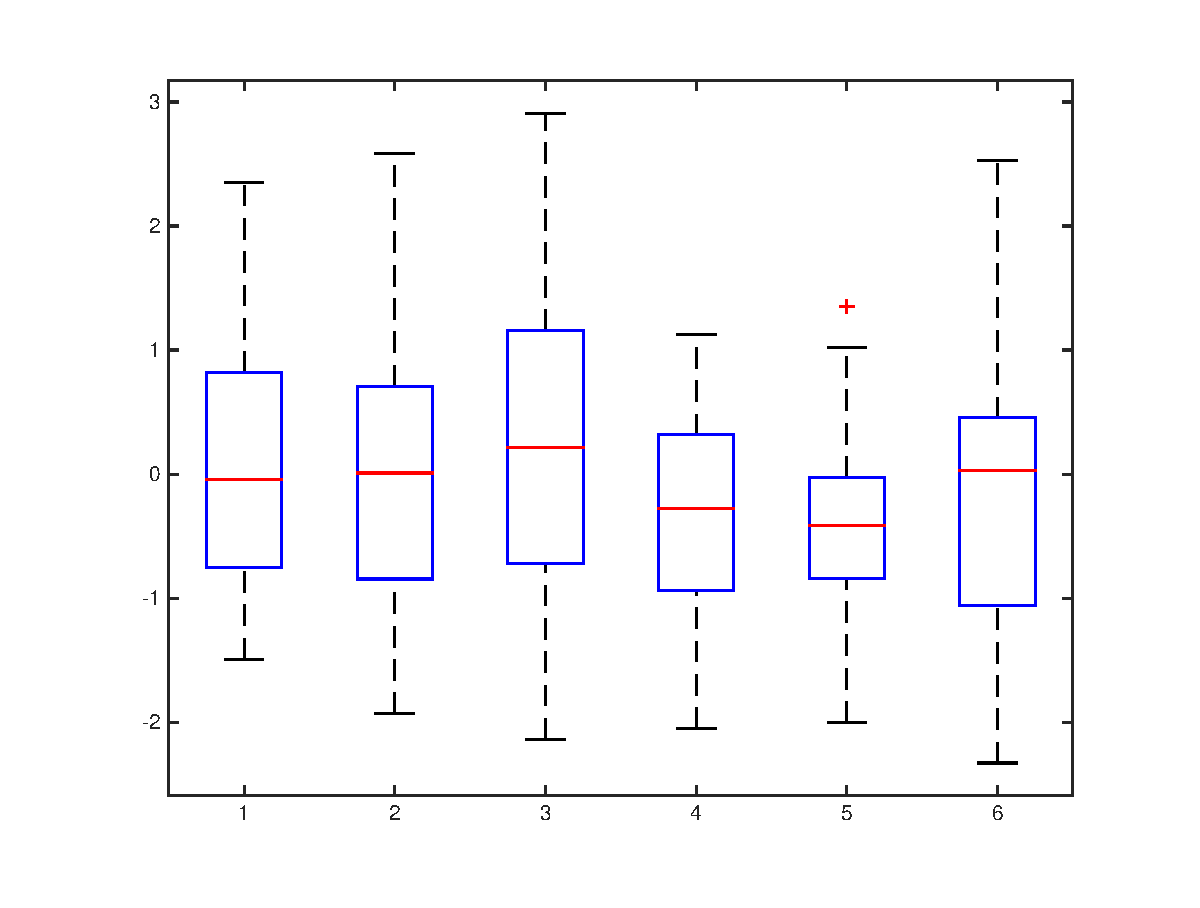
\includegraphics[width=0.75\textwidth]{cc.eps}
%	\caption{Correlation Coefficients \& Time}
%	\label{fig:boxplot}
%\end{figure*}

%TODO boxplots - high curvature shapes are harder to make.

%fig9
\begin{figure*}
	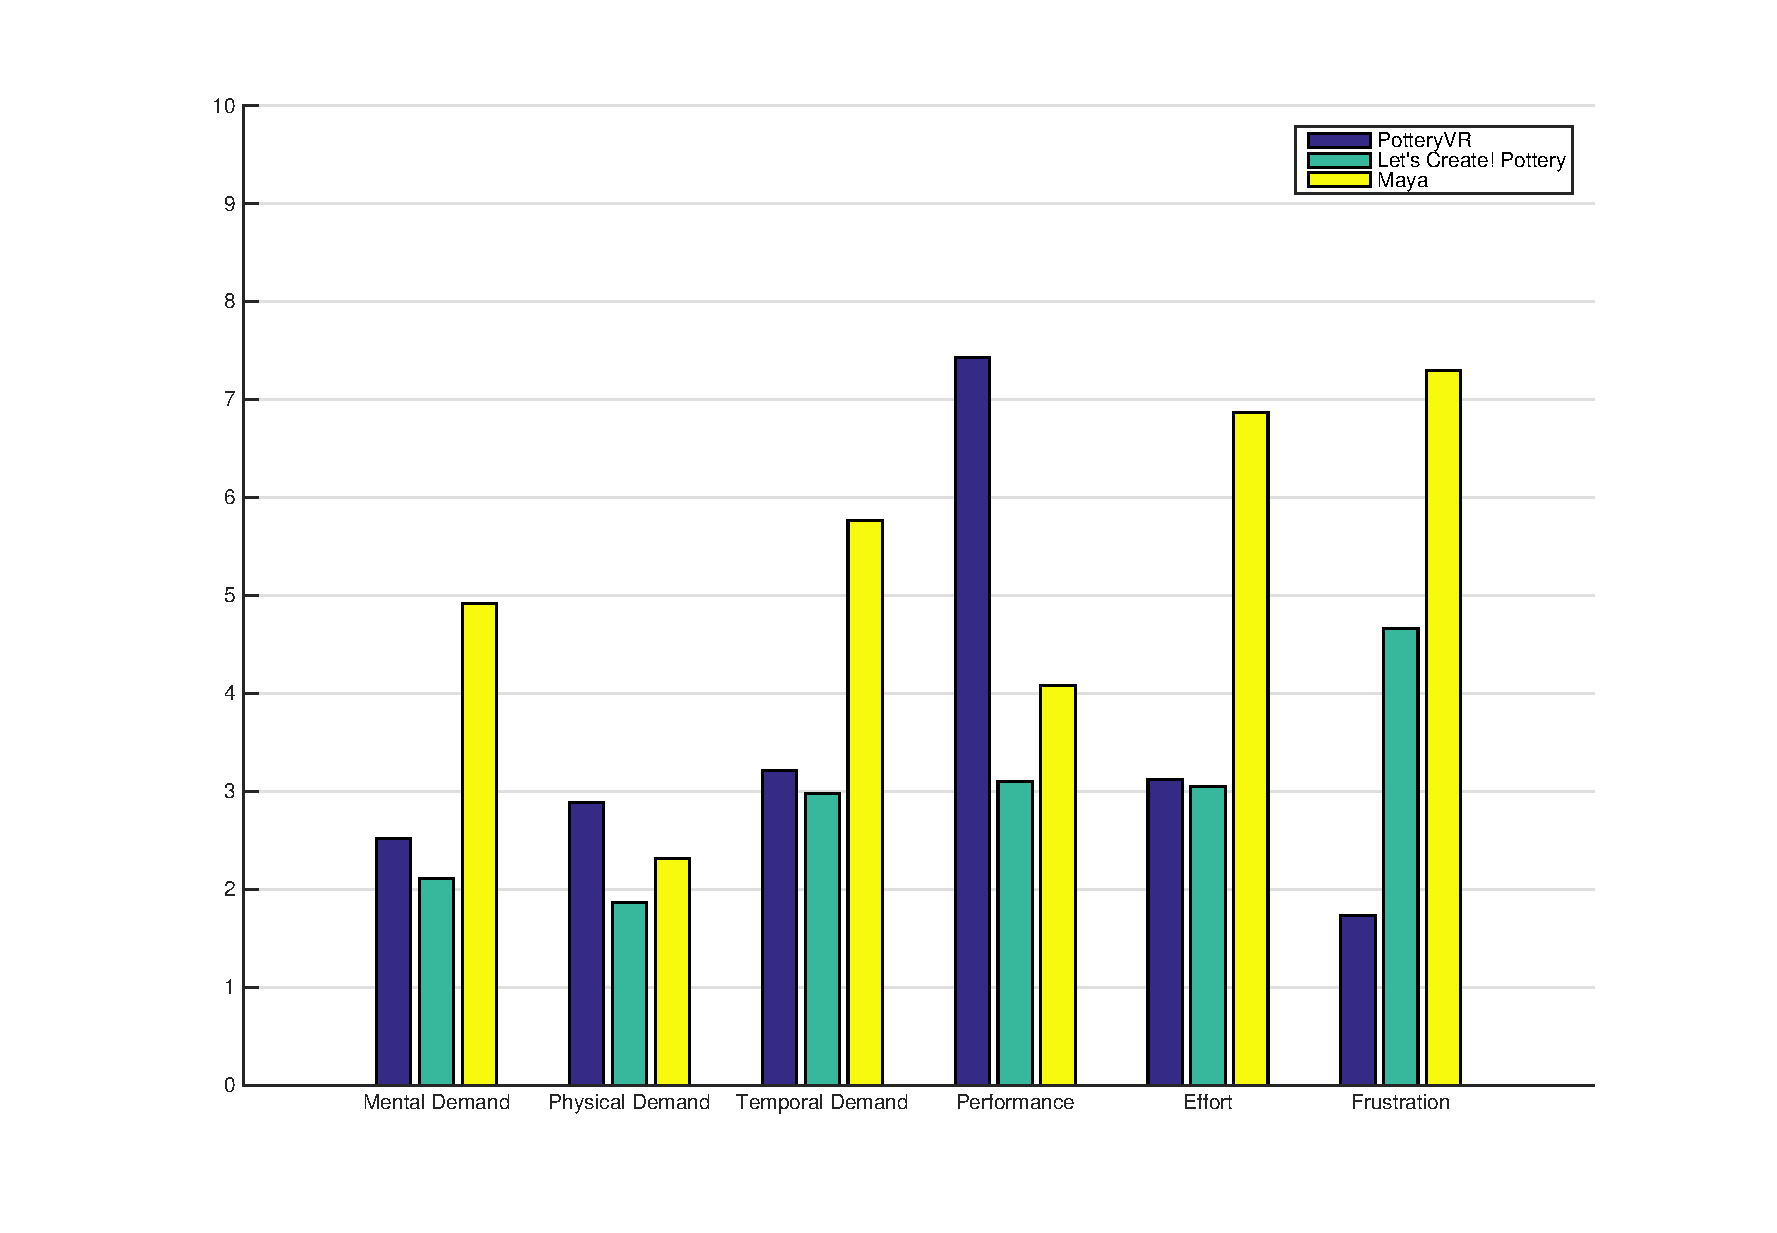
\includegraphics[width=\textwidth]{tlx.eps}
	\caption{Mean values of the six dimensions of NASA-TLX.}
	\label{fig:tlx}
\end{figure*}

%mental/physical/temporal
According to Figure \ref{fig:tlx}, we can get some findings. 
Firstly, the mental demand values of T1 (M = 2.52) and T2 (M = 2.11) were almost the same and much lower than the value of T3 (M = 4.92). Similarly, the temporal demand value of T3 (M = 5.77) was much higher than the values of T1 (M = 3.21) and T2 (M = 2.98). This indicated that EasyPot and LCP were easier to use and less time-consuming than Maya. Unsurprisingly, the physical demand value of T1 (M = 2.89) is slightly higher than T2 (M = 1.86) and T3 (M = 2.31), which means interactions based spatial movements are slightly laborious than touchscreen and keyboard/mouse interactions.

%[Maya - hard]
Maya showed much higher values in effort (M = 6.87) and frustration (M = 7.30) and lower value in performance (M = 4.08) compared with EasyPot and LCP.
Since most subjects in the user study have no 3D modeling software experience, the complex user interface in Maya makes it challenging for these novice users to memorize where to find the commands they need, rendering a high effort.
Although keyboard-mouse based interaction allows precise controls with low physical demand, many subjects struggled with selecting and manipulating vertices and faces accurately, which caused high user frustration. As a result, most subjects were not satisfied with their performances in T3.

%[LCP - limitation] [thickness smooth sharpness]
Surprisingly, we found that it was not as satisfied as we predicted for the subjects using LCP in T2, where the performance value (M = 3.10) is lower than we expected. This is due to the limitations in LCP: Although the interaction in LCP is easy to learn, some high curvature features (Figure \ref{fig:target}b, \ref{fig:target}d, \ref{fig:target}e and \ref{fig:target}f) cannot be reached due to LCP has a fixed deformation range. Moreover, subjects cannot modify the thickness of pots, which is another limitation of LCP. Thus, the frustration value (M = 4.66) are high during T2.

%fig10
\begin{figure*}
	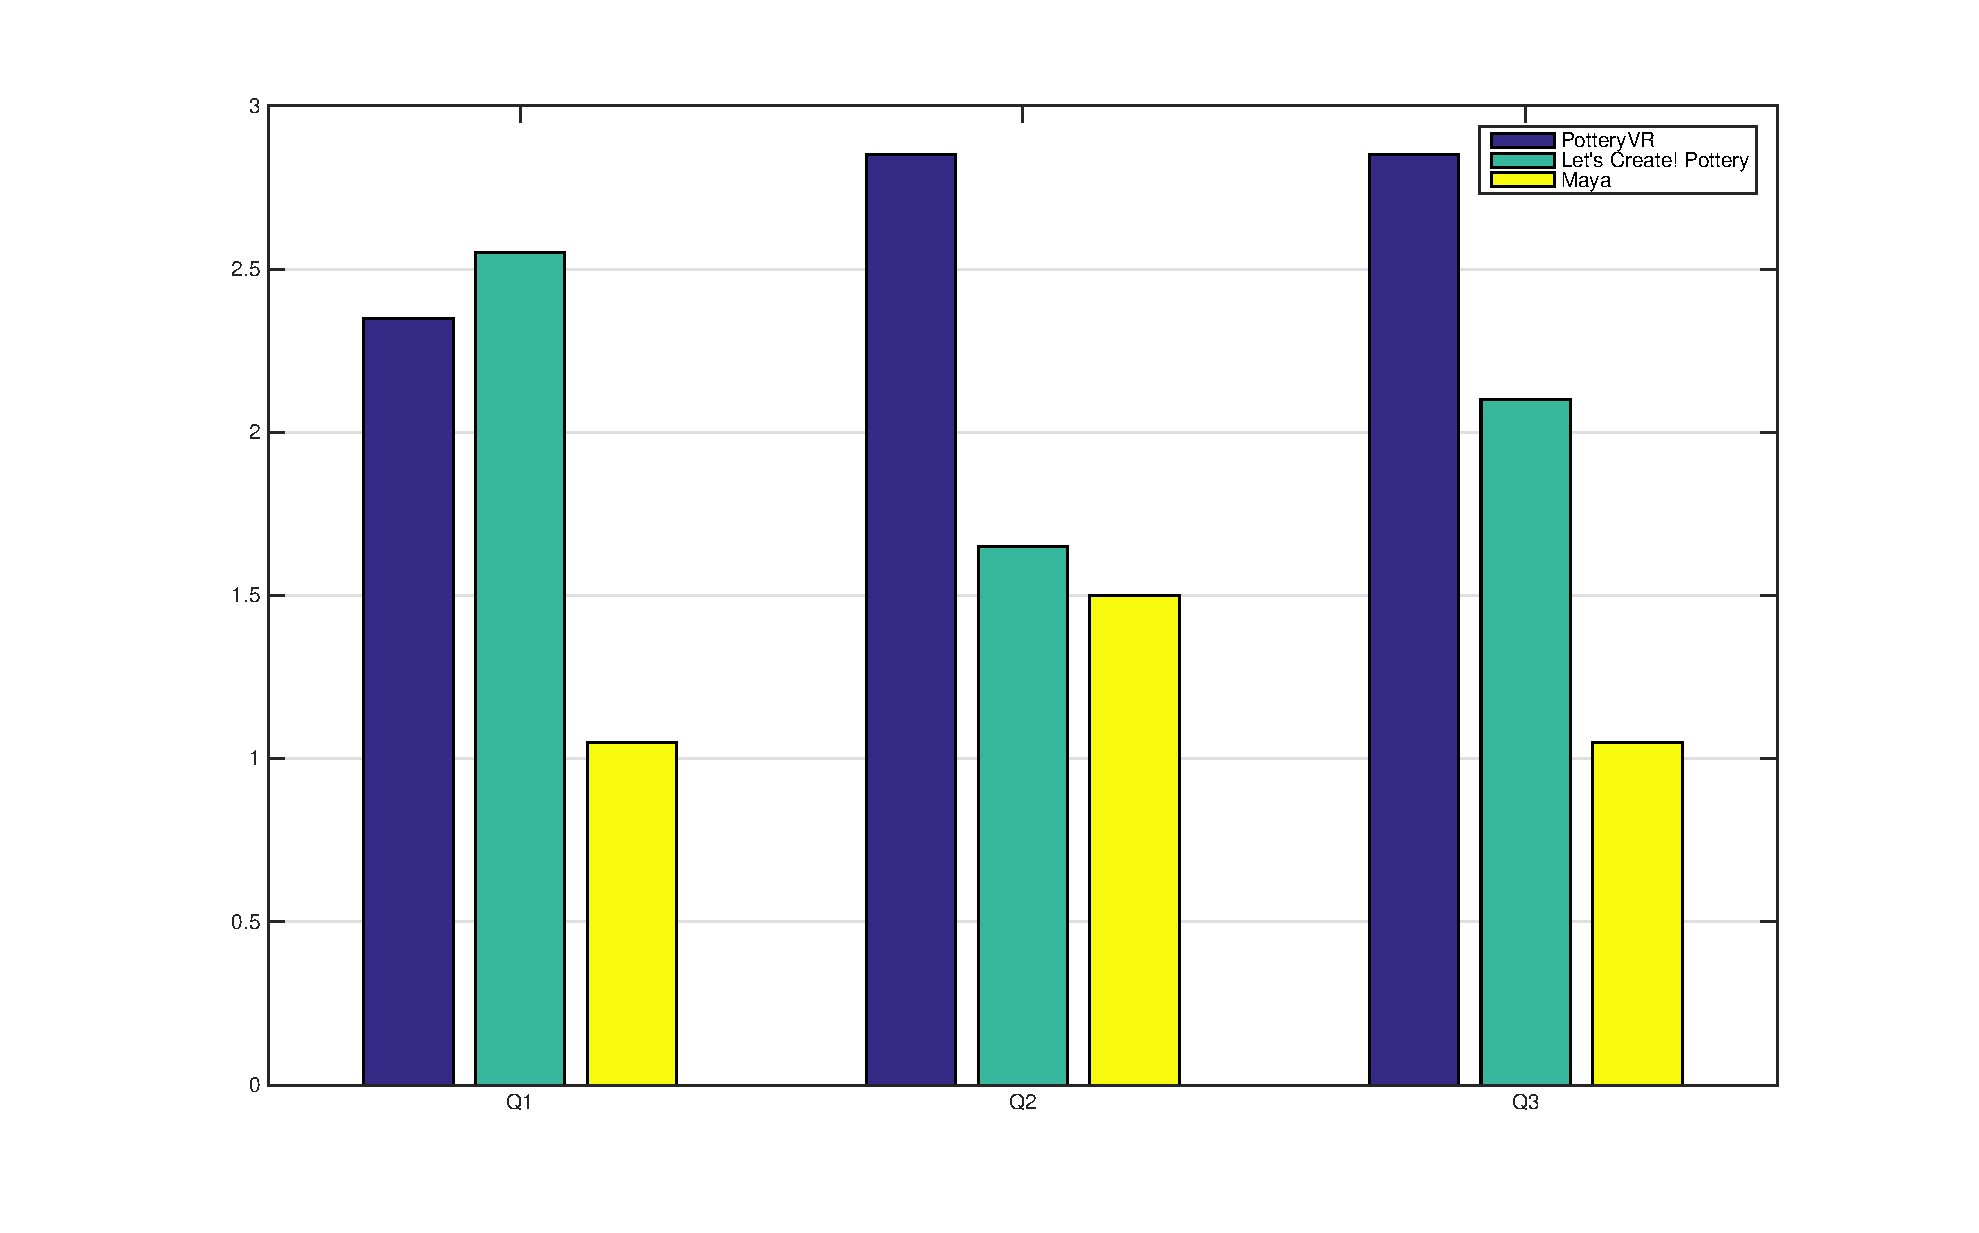
\includegraphics[width=0.75\textwidth]{ranking.eps}
	\caption{Mean ranking scores of Q1, Q2 and Q3.}
	\label{fig:ranking}
\end{figure*}

%[user preference][enjoyable and intuitive]
The voting results in Figure \ref{fig:ranking} demonstrated the ease of learning, the support of creativity and overall preference of the three systems.
%ease
Compared with the complex interfaces and the keyboard and mouse operations in Maya, EasyPot and LCP provides simple interfaces and intuitive interactions, allowing users get familiar with the interaction with ease.
%creativity
In addition, most subjects considered EasyPot stimulate their creativity and imagination the most. From their feedbacks, we found that spatial interactions in virtual reality context gave them a novel and realistic way to interact with virtual clay when using EasyPot. Moreover, EasyPot provides more powerful operations such as adjustable deformation range, thickness control and smoothing than LCP, allowing subjects creating characteristic shapes.

%overall-enjoyable, useful for training
In Q3, EasyPot became the favorite virtual pottery system for the subjects. From user feedbacks, we found that EasyPot provided the subjects with most enjoyable experience among the three systems, which also has a balance of having simple interfaces and useful functionalities. In addition, the natural bimanual interactions in EasyPot are closely related to the operations in reality pottery, making it an ideal training simulation tool for pottery.

\section{Discussions}
\label{sec:7}
%[Positive]
We collected user feedbacks after the subjects had used our system. In summary, subjects gave many positive feedbacks when using our system to design pottery models. They spoke highly of the immersive pottery creation experience with intuitive interaction and haptic feedback that motivated them to design potteries just like working on real clay. In addition, the undo/redo are quite convenient according to the subjects, which enhances the efficiency during the creation process. For those who have no real life pottery creation experience enjoyed our system very much and would like to try real pottery someday. 

%[Suggestions]
During our user study, we found that the undo/redo functionality is not used frequently as we expected. 
We also asked their suggestions for the future features they wanted to see in EasyPot.
A few subjects expressed their wishes to add coloring feature, which allows them decorate the pots with colors and patterns.
At the end of our user study, many subjects said they would like to try EasyPot one more time.

%[limitations]
Our system still has its limitations. First, the physical size of the motion controllers sometimes influence the deformation in bimanual mode, especially when the part of the clay is narrow that two controllers may collide with each other. For example, when subjects working on the neck of clay, it will be difficult to edit with two controllers. This problem can be easily solved by providing user one-hand deformation mode. We plan to use data gloves to avoid these situations in the future.
%
Second, the potteries designed by our systems lack colors and textures. Although we focus on deformation in our study, several subjects stated that they wish to paint the pottery after designing the shape of the clay. We intend to add new features related to interactive painting on 3D objects.
%
Another limitation of our system is that it cannot adding handles to the pottery. We will introduce more tools that allow users to modify the topology of the mesh in order to create more personalized pottery works.


\section{Conclusions}
\label{sec:8}

We present EasyPot, a realtime pottery modeling system in Virtual Reality.
Closely linked to the pottery creation experience real life, our system enables users to manipulate the mesh in realtime with two hands, allowing them creating a variety of pottery models from realistic generated clay meshes.
As an educational tool, EasyPot can help novice users to learn real life pottery creation process in virtual environment, who can fabricate their works using our system with a 3D printer.
Our results have shown that EasyPot has relative advantage compared with traditional desktop 3D modeling experience (Maya) and touchscreen experience (Let's Create! Pottery).
A possible extension of our system is to support interactive coloring functionalities in the future, which can enhance the artistry of user generated pottery works.


\begin{acknowledgements}
%If you'd like to thank anyone, place your comments here
%and remove the percent signs.
\end{acknowledgements}

% BibTeX users please use one of
%\bibliographystyle{spbasic}      % basic style, author-year citations
\bibliographystyle{spmpsci}      % mathematics and physical sciences
%\bibliographystyle{spphys}       % APS-like style for physics
\bibliography{pottery}   % name your BibTeX data base

% Non-BibTeX users please use
%\begin{thebibliography}{}
%
% and use \bibitem to create references. Consult the Instructions
% for authors for reference list style.
%
%\bibitem{RefJ}
% Format for Journal Reference
%Author, Article title, Journal, Volume, page numbers (year)
% Format for books
%\bibitem{RefB
%Author, Book title, page numbers. Publisher, place (year)
% etc
%\end{thebibliography}

\end{document}
% end of file template.tex

